\chapter{\heiti \label{ch2}技术背景知识}
\section{\heiti model}

\begin{figure}[thb]
  \centering
    \subfigure{
      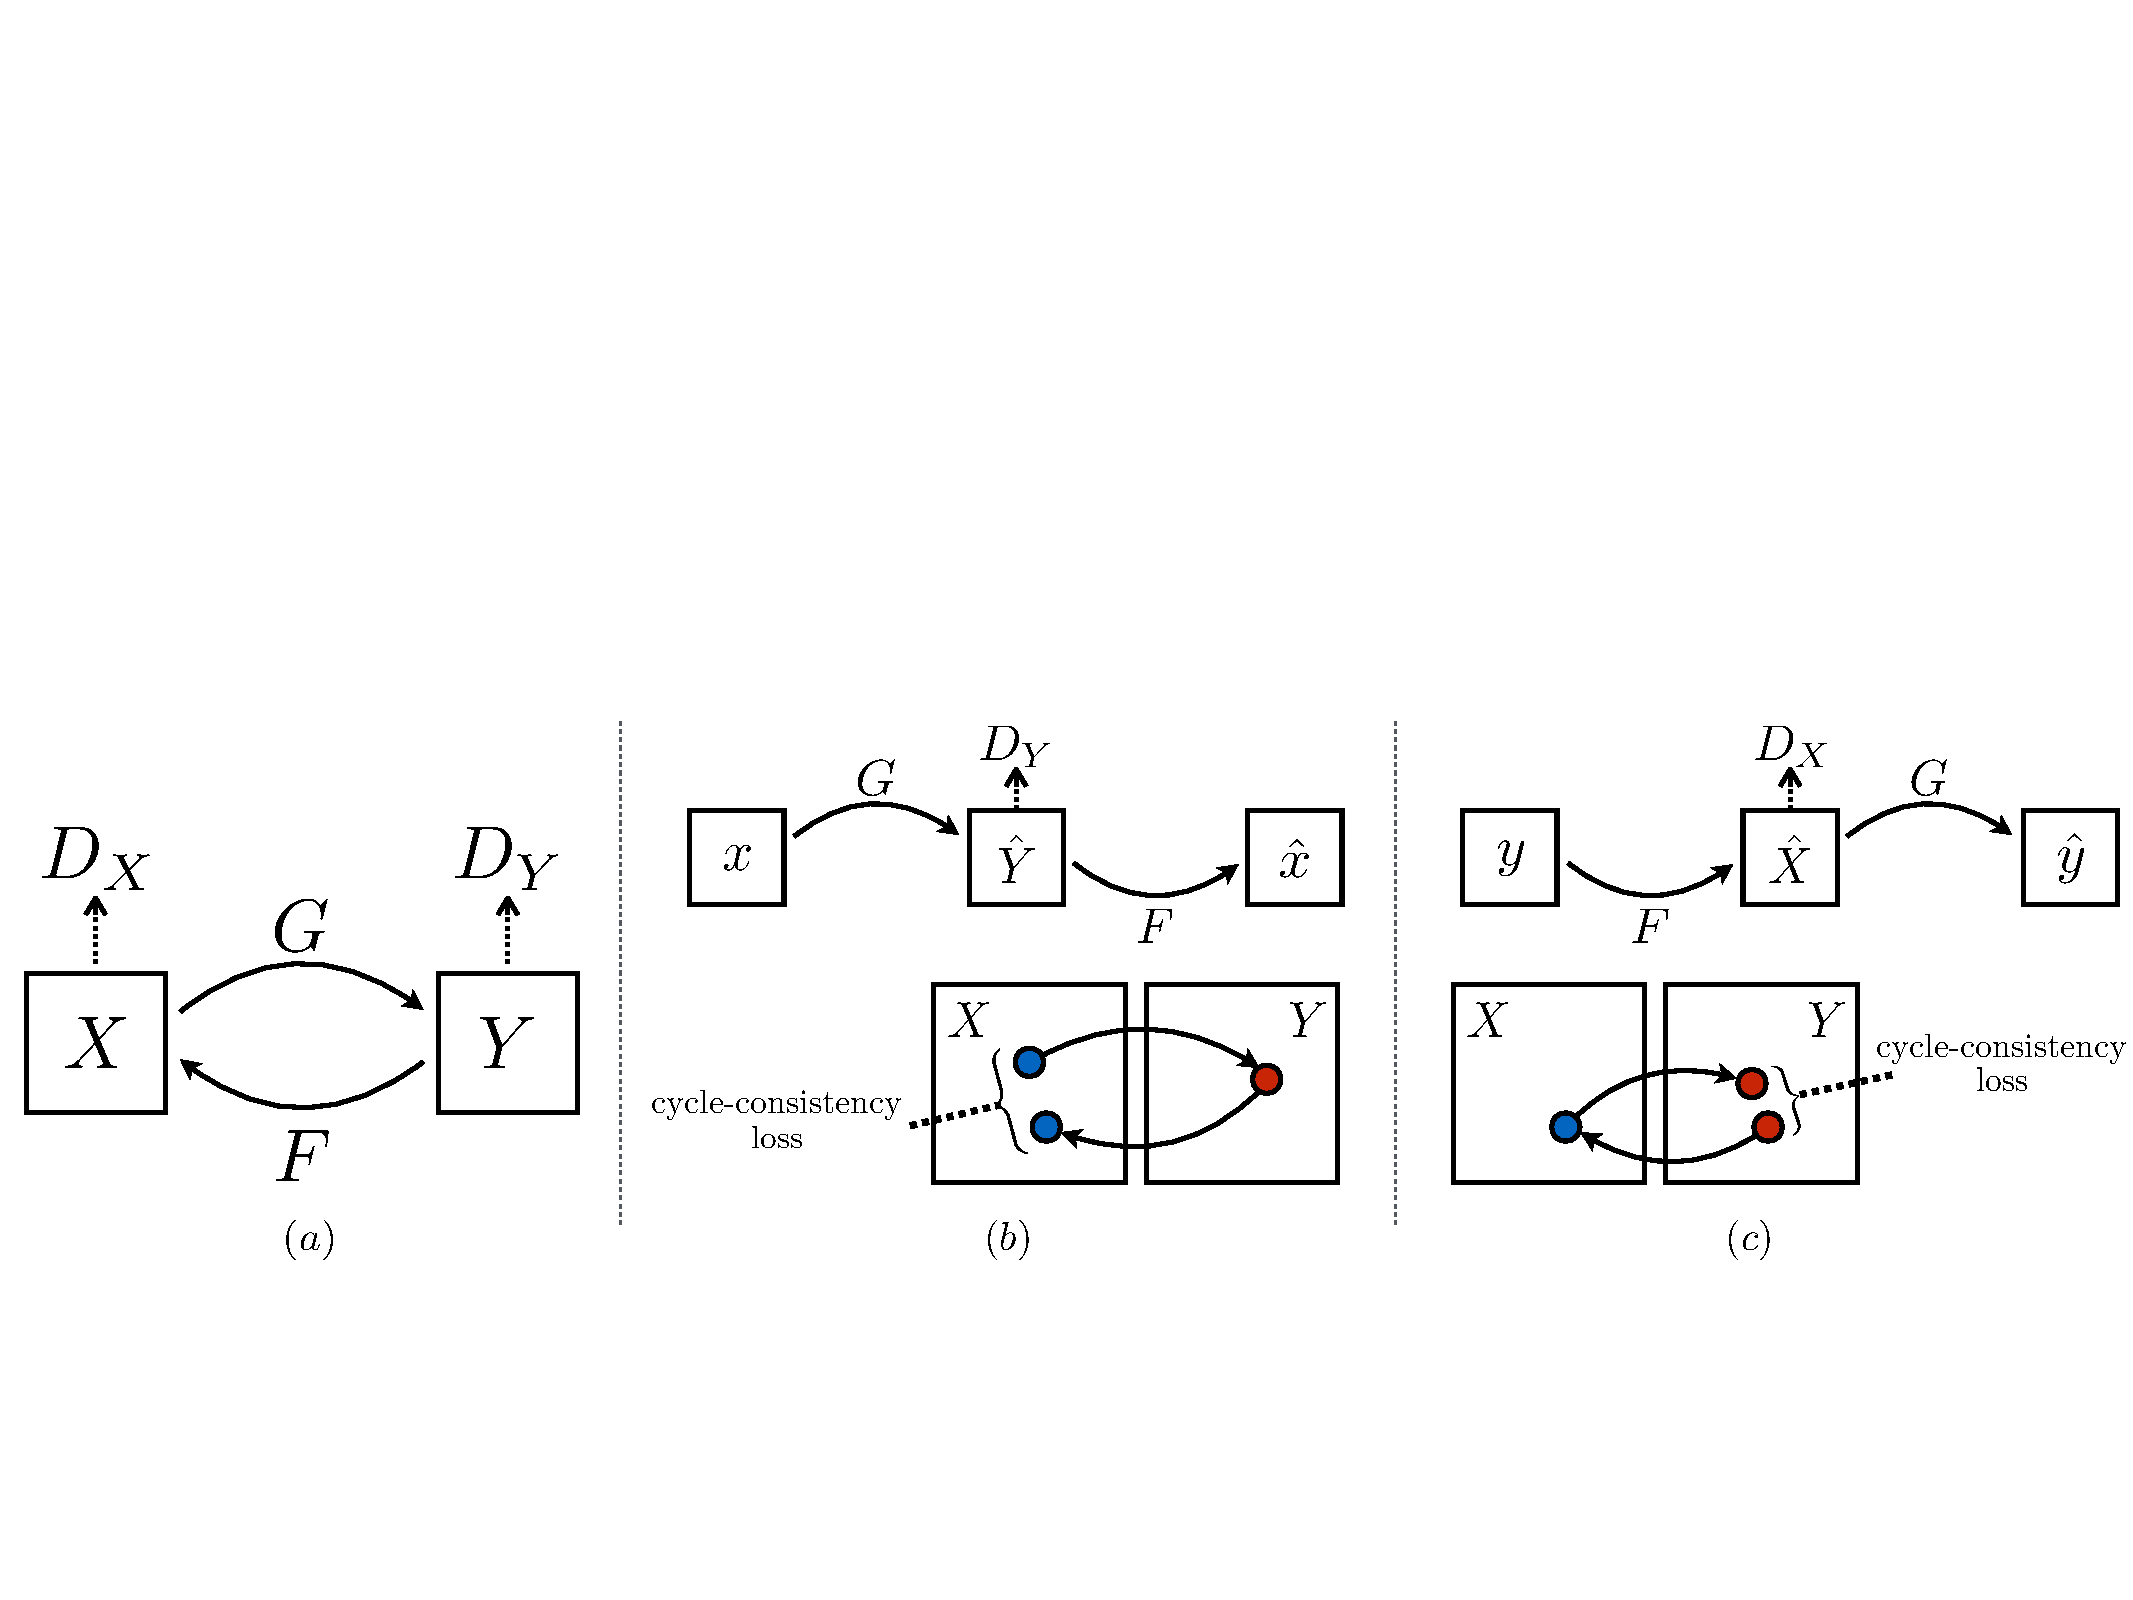
\includegraphics[width=0.9\textwidth]{images/system_diagram_v2.pdf}}
  \caption{CycleGAN is actually an A→B one-way GAN plus a B→A one-way GAN. The two GANs share two generators, each with a discriminator, so adding up to a total of two discriminators and two generators. A one-way GAN has two losses, and CycleGAN adds up to a total of four losses.}
  \label{fig:PGM1}
  \end{figure}

\subsection{\heiti 表示}
Adversarial Loss:For the mapping function G : X → Y and its dis- criminator DY , we express the objective as

\begin{align}
\mathcal{L}_{\text{GAN}}(G,D_Y,X,Y) =  \ \mathbb{E}_{y \sim p_{\text{data}}(y)}[\log D_Y(y)] \nonumber \\
+  \ \mathbb{E}_{x \sim p_{\text{data}}(x)}[\log (1-D_Y(G(x))]
\end{align}

\begin{align}
  \mathcal{L}_{\text{GAN}}(G,D_X,X,Y) =  \ \mathbb{E}_{x \sim p_{\text{data}}(y)}[\log D_X(y)] \nonumber \\
  +  \ \mathbb{E}_{y \sim p_{\text{data}}(x)}[\log (1-D_X(G(x))]
  \end{align}

  Cycle Consistency Loss. The so-called Cycle consistency is to ensure
  
  Forward consistent: x->G(x)->F(G(x))≈x
  
  Backward agreement: y->F(y)->G(F(y))≈y

  We incentivize this behavior using a cycle consistency loss:
 \begin{align}
   \mathcal{L}_{\text{cyc}}(G, F) =  mathbb{E}_{x\sim p_{\text{data}}(x)} [[{F(G(x))-x}]_1] \nonumber \\ 
   + \ \mathbb{E}_{y\sim p_{\text{data}}(y)}[[{G(F(y))-y}]_1]
 \end{align}

 full objective loss function is:
 \begin{align}
  \mathcal{L}(G,F,D_X,D_Y) = \mathcal{L}_{\text{GAN}}(G,D_Y,X,Y) \nonumber \\
  +\ \mathcal{L}_{\text{GAN}}(F,D_X,Y,X) \nonumber \\
  +\  \lambda \mathcal{L}_{\text{cyc}}(G, F)
 \end{align}




\section{\heiti 深度生成模型}
The network architecture of CycleGAN is shown in the figure\ref{fig:1}:

  \begin{figure}
  \centering
\subfigure[]{
  \begin{minipage}[b]{0.9\textwidth}
  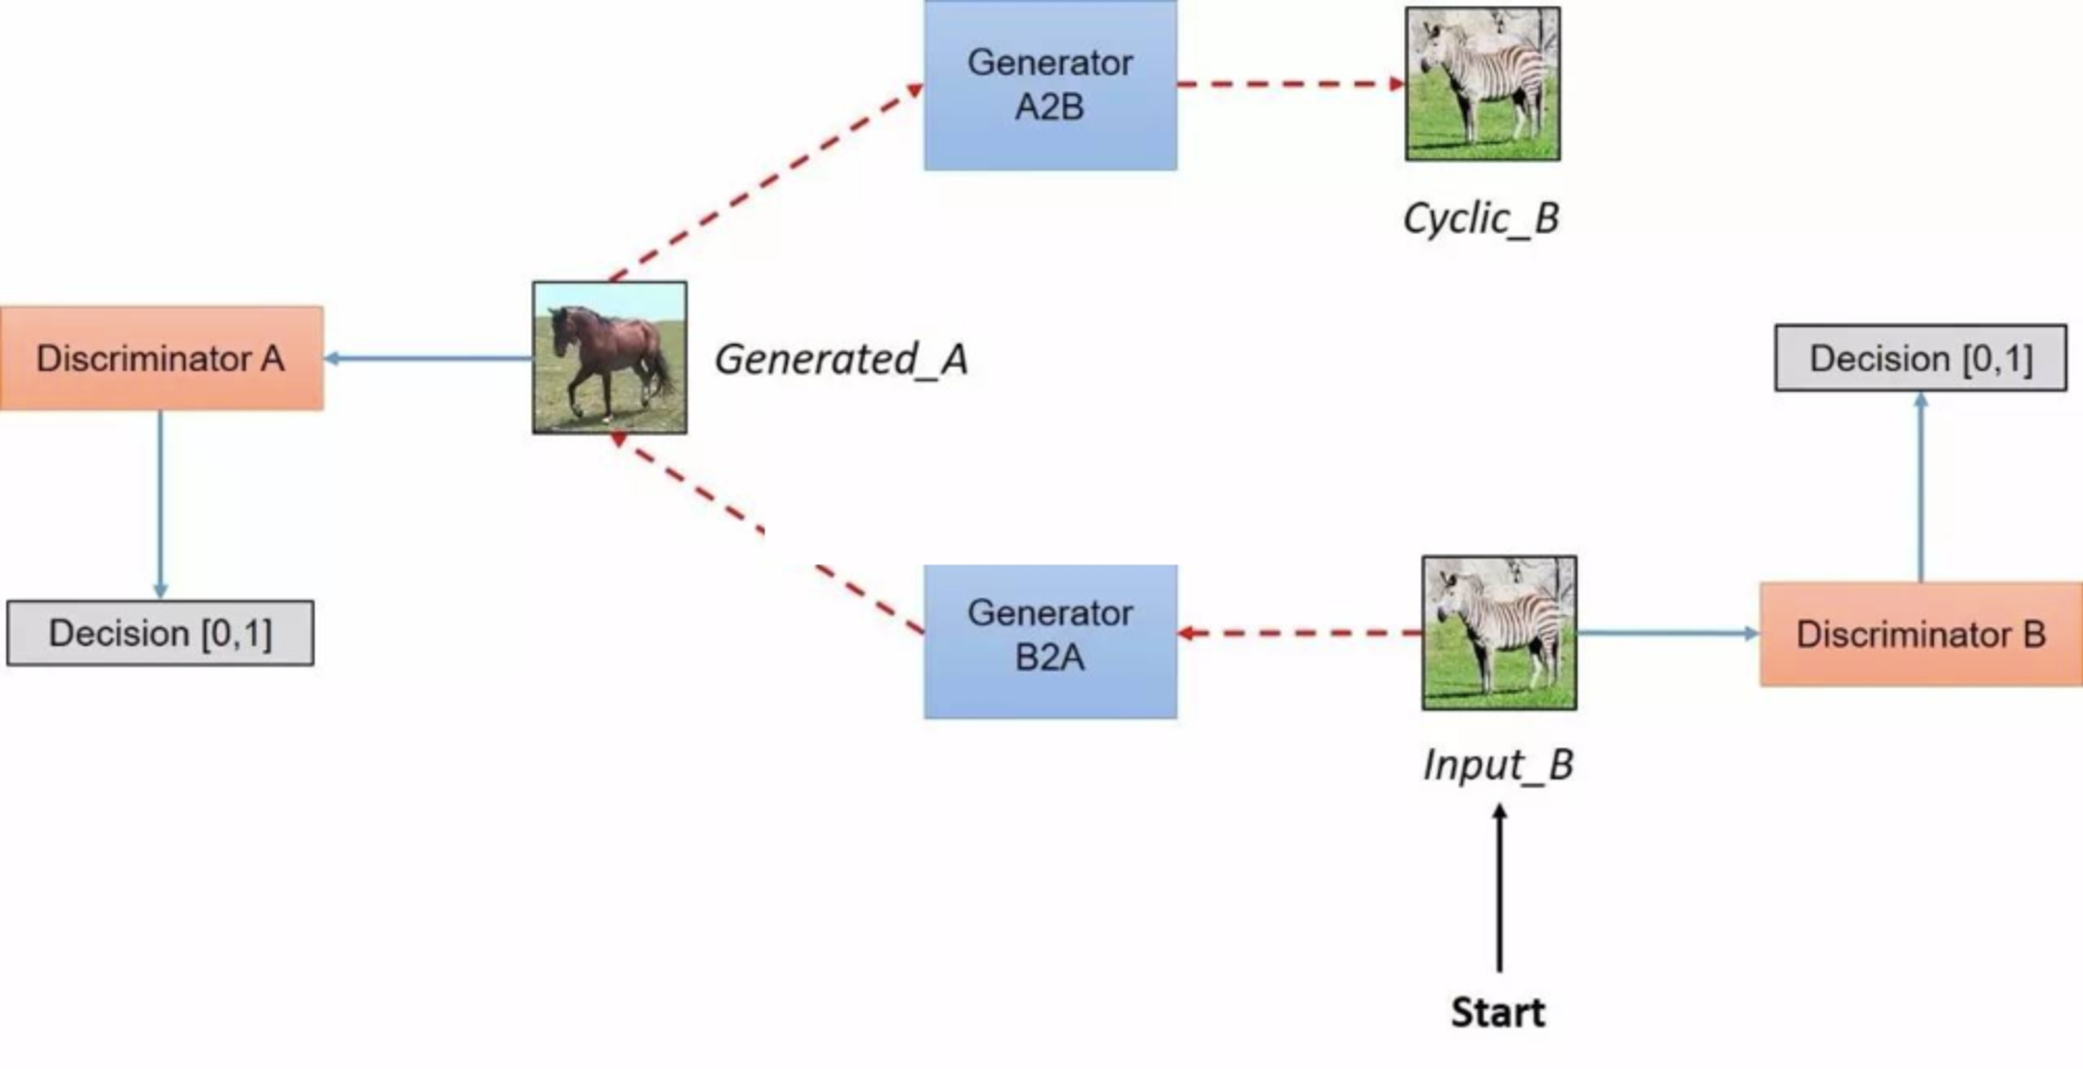
\includegraphics[width=1\textwidth]{images/agr.pdf}
\end{minipage}}
\subfigure[]{
  \begin{minipage}[b]{0.9\textwidth}
  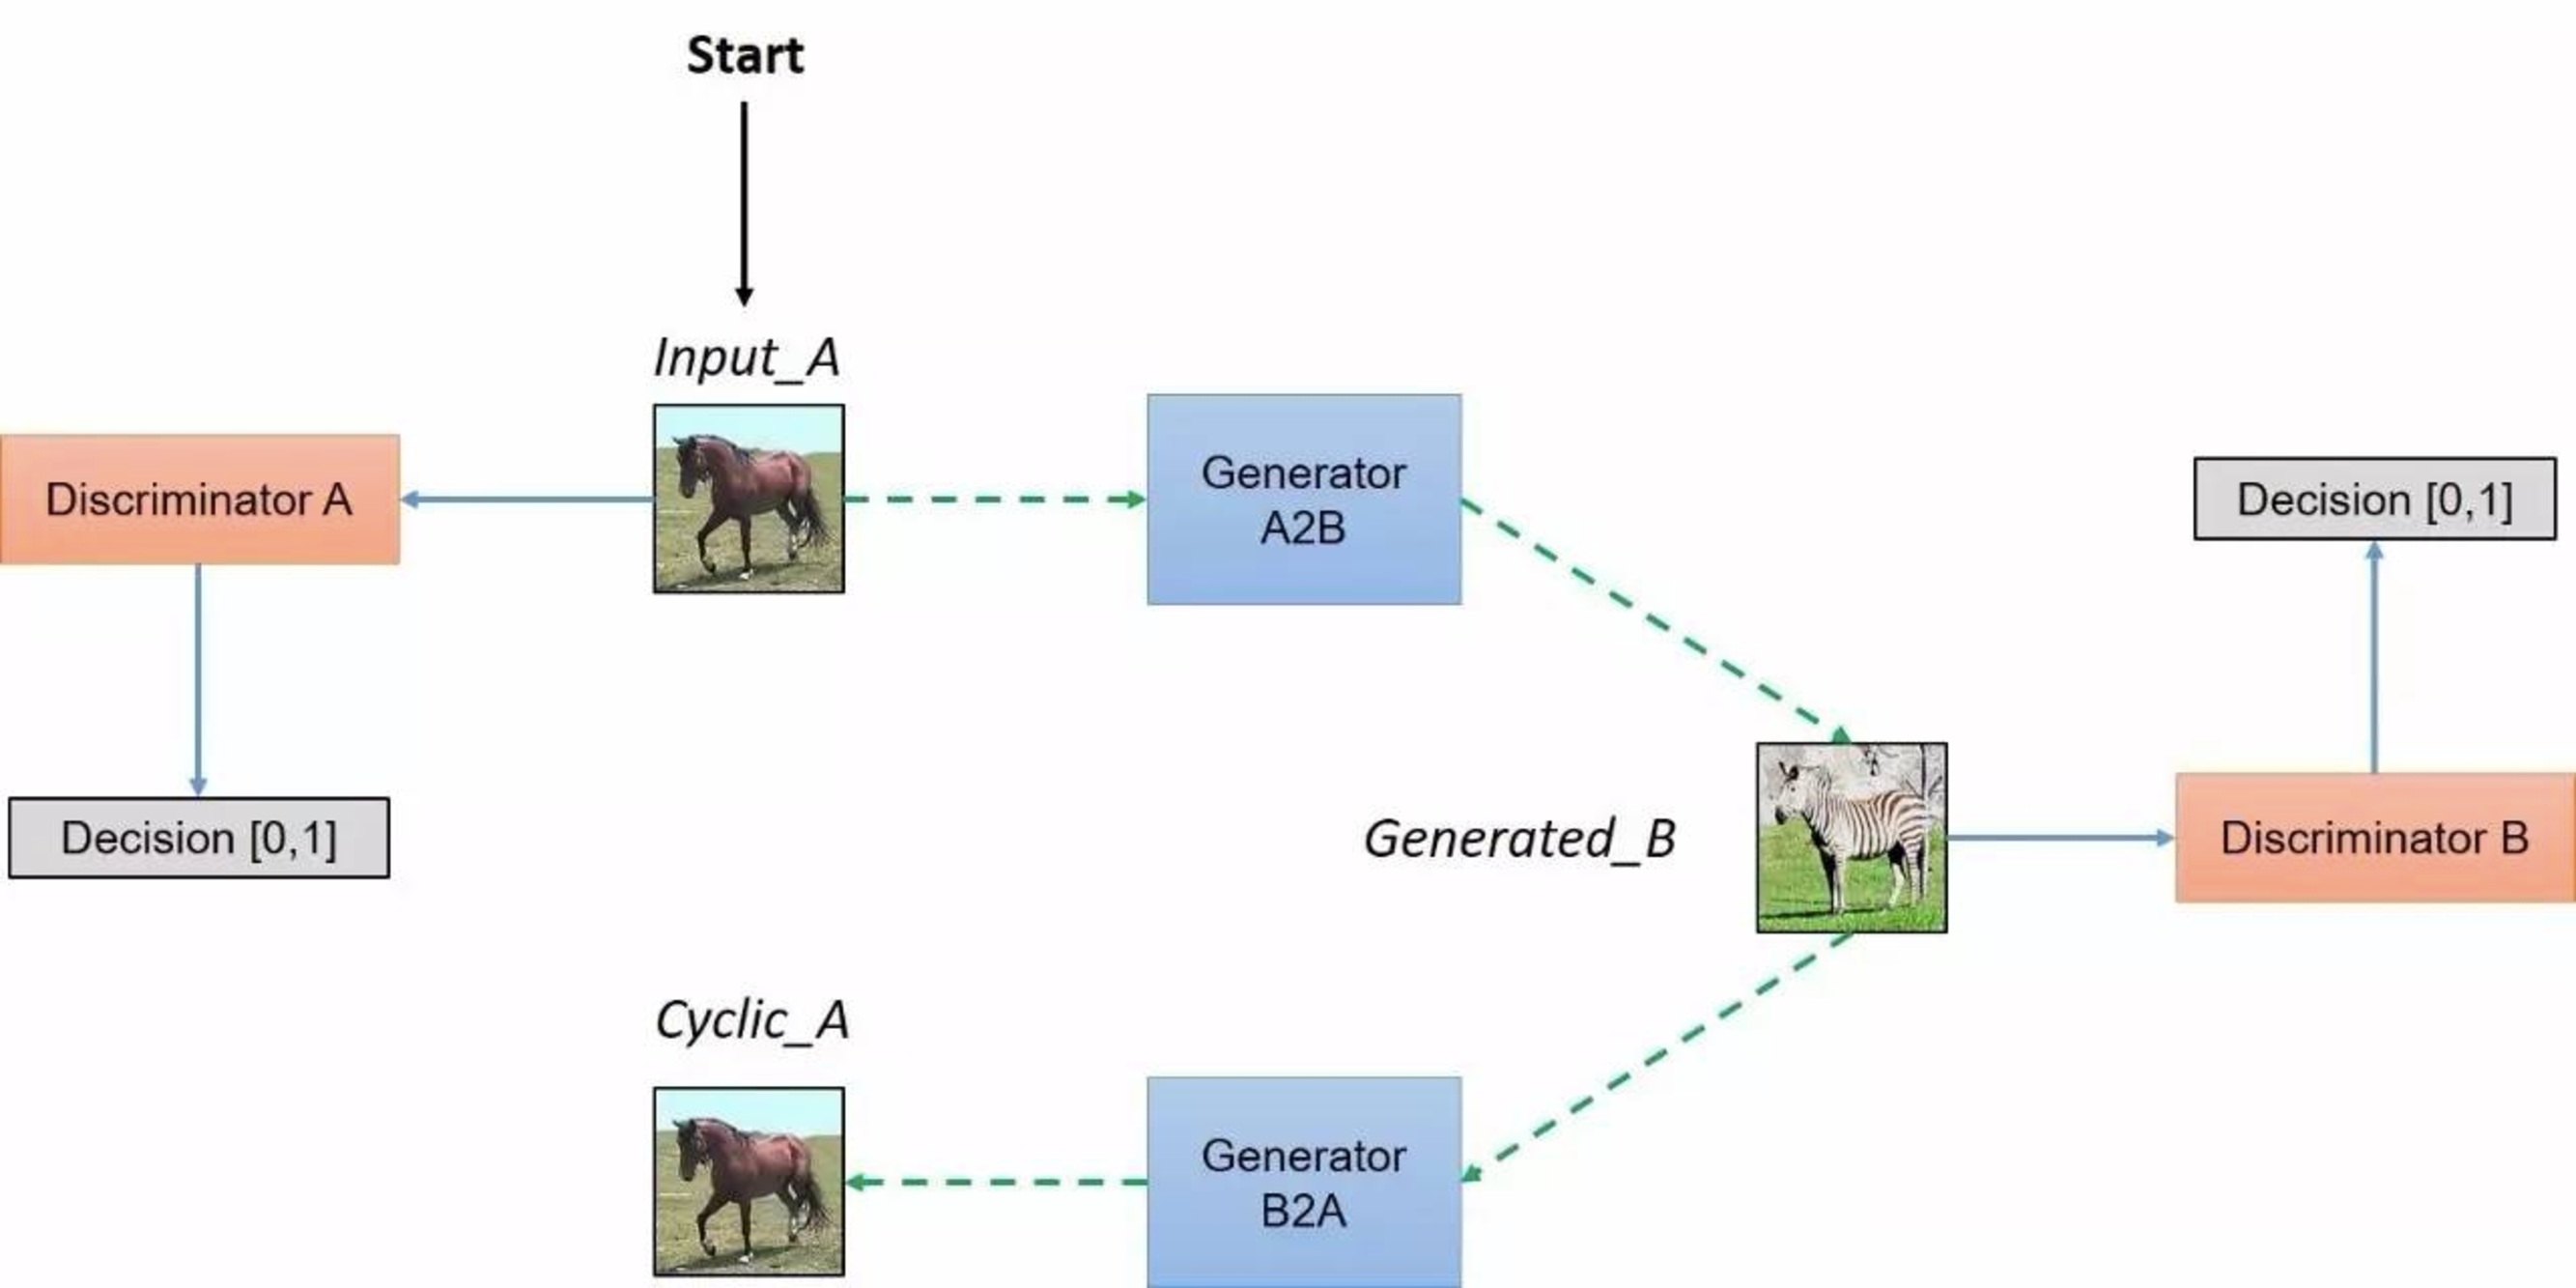
\includegraphics[width=1\textwidth]{images/agr1.pdf}
\end{minipage}} 
\caption{The model acquires an input image from the domain DA, 
which is passed to the first generator GeneratorA→B, 
whose task is to convert a given image from the 
domain DA to an image in the target domain DB. 
This newly generated image is then passed to another generator, 
GeneratorB→A, whose task is to convert back to 
the image CyclicA in the original domain DA,
which can be compared to the autoencoder. 
This output image must be similar to the 
original input image and is used to define 
meaningful mappings that did not exist in the unpaired data set.} 
\label{fig:1}
\end{figure}

    